\sectionthree{NFA State Diagram}
\begin{python0}
  from solutions import *; clear()
\end{python0}

The following is a
\defone{state diagram} or 
\tinysidebarskip\defone{transition diagram}
of a
\defone{nondeterministic finite state automata NFA}
Some people also called the device a
\sidebarskip{24pt}
\defone{nondeterministic finite state machine NFSM}.
\sidebarskip{0pt}

\begin{center}
\begin{tikzpicture}[shorten >=1pt,node distance=2cm,auto,initial text=,
initial where=above]
\node[state,initial]   (q0) [shape=circle, draw] at ( 0,  0) {$q_0$};
\node[state]           (q1) [shape=circle, draw] at (-1, -4) {$q_1$};
\node[state]           (q3) [shape=circle, draw] at ( 1, -2) {$q_3$};
\node[state,accepting] (q4) [shape=circle, draw] at ( 1, -4) {$q_4$};
\node[state,accepting] (q2) [shape=circle, draw] at (-1, -6) {$q_2$};

\path[->]
(q0) edge [loop right] node {$a,b$} ()
(q0) edge node {$b$} (q1)
(q0) edge node {$\epsilon$} (q3)
(q1) edge node {$b$} (q2)
(q3) edge node {$\epsilon$} (q1)
(q3) edge node {$a$} (q4)
;
\end{tikzpicture}\end{center}


An edge labeled with symbol $a$ is called an
\defone{$a$--transition}.


%-*-latex-*-

\begin{ex} 
  \label{ex:prob-00}
  \tinysidebar{\debug{exercises/{disc-prob-28/question.tex}}}

  \solutionlink{sol:prob-00}
  \qed
\end{ex} 
\begin{python0}
from solutions import *
add(label="ex:prob-00",
    srcfilename='exercises/discrete-probability/prob-00/answer.tex') 
\end{python0}


This is how you use the machine. It's very similar to the state
diagram of a DFA except that you keep track of a
\textbf{set} of states
instead of just one.

\begin{itemize}
  \item[(1)] Start at the \textbf{start state}.
   This is the same as DFA. Look for it now. Keep track of this
   state.
 \item[(2)] Read the first character of the string; you always
 \textbf{start from the left} of the string and
 \textbf{move right}.
 \item[(3)] Go from the node you're pointing at to the
 \textbf{nodes}
 (there might be more than one!)
 using
 the \textbf{edges} labeled with the character you've just read.
 Note that you might have more than one path!
 \item[(4)] If there are $\ep$-transition, you need to keep the
  states
 you can get to via these $\ep$-transitions too.
 \item[(5)] If a path cannot have a transition, that path dies.
 \item[(6)] Repeat the above process (2)-(3) until you have no more characters.
 \item[(7)]
   An
   \defone{accept state}
   is a node with a double-circle boundary.
   It's also called a
   \defone{final state}.
   When you have finished scanning your string left to right,
   you will have a set of paths.
   If there is a path that ends in an accepting state, then the
   string is accepted.
\end{itemize}


Now let's execute our NFA for several different words $w$. 
Let's call the above NFA $N_1$.

\begin{center}
\begin{tikzpicture}[shorten >=1pt,node distance=2cm,auto,initial text=,
initial where=above]
\node[state,initial]   (q0) [shape=circle, draw] at ( 0,  0) {$q_0$};
\node[state]           (q1) [shape=circle, draw] at (-1, -4) {$q_1$};
\node[state]           (q3) [shape=circle, draw] at ( 1, -2) {$q_3$};
\node[state,accepting] (q4) [shape=circle, draw] at ( 1, -4) {$q_4$};
\node[state,accepting] (q2) [shape=circle, draw] at (-1, -6) {$q_2$};

\path[->]
(q0) edge [loop right] node {$a,b$} ()
(q0) edge node {$b$} (q1)
(q0) edge node {$\epsilon$} (q3)
(q1) edge node {$b$} (q2)
(q3) edge node {$\epsilon$} (q1)
(q3) edge node {$a$} (q4)
;
\end{tikzpicture}\end{center}


First let me run $N_1$ on $w = \epsilon$. We start $N_1$ at $q_0$. 
\begin{enumerate}
\li $N_1$ stops immediately at $q_0$ since there is no character to process.
\li However $N_1$ is greedy and sees that it can also go to state $q_3$
\textit{without} processing any character (from the input):
    there's a transition from $q_0$ to $q_3$ labeled $\epsilon$.
    So it spawns a copy of itself, say $N_2$, at state $q_3$ while
    it stays at $q_0$.
    Note that $N_2$ is an exact copy of $N_1$ -- it behaves the say
    way and it has the exact same input as $N_1$. 
    The new machine $N_2$ is at state $q_3$ and stops there since there's
    nothing to process and $N_2$ cannot spawn a new copy of itself.
\li However $N_2$ being just as greedy as $N_1$,
    sees that it can also go to $q_1$ without processing any character.
    So $N_2$ stays at $q_3$ while it spawns off another machine, 
    say $N_3$, at state $q_1$ while $N_2$ stays at $q_3$.
    $N_3$ stops at state $q_1$. 
\end{enumerate}
At this point, all machines stops processing characters and 
they have spawn the maximum number of machines along 
$\epsilon$-transitions. 
Everyone (everyit?) now reports their states to $N_1$ and disappears.
$N_1$ looks at all the states that all of its descendents (and itself) have
reached.

\begin{center}
\begin{tikzpicture}[shorten >=1pt,node distance=2cm,auto,initial text=,
initial where=above]
\node[state,initial,fill=blue!10]   (q0) [shape=circle, draw] at ( 0,  0) {$q_0$};
\node[state,fill=blue!10] (q1) [shape=circle, draw] at (-1, -4) {$q_1$};
\node[state,fill=blue!10] (q3) [shape=circle, draw] at ( 1, -2) {$q_3$};
\node[state,accepting] (q4) [shape=circle, draw] at ( 1, -4) {$q_4$};
\node[state,accepting] (q2) [shape=circle, draw] at (-1, -6) {$q_2$};

\path[->]
(q0) edge [loop right] node {$a,b$} ()
(q0) edge node {$b$} (q1)
(q0) edge node {$\epsilon$} (q3)
(q1) edge node {$b$} (q2)
(q3) edge node {$\epsilon$} (q1)
(q3) edge node {$a$} (q4)
;
\end{tikzpicture}\end{center}

None of the $3$ machine manage to reach an accepting state.
So $N_1$ does not accept (i.e rejects) $\epsilon$.


Now let me run $N_1$ on $w = a$. Again I start $N_1$ at $q_0$.
\begin{enumerate}
  \li $N_1$ begins at state $q_0$. It's about to process $a$,
  but before it does that ...
  \li $N_1$ is greedy and spawns another machine $N_2$ which is at state $q_3$
  because there's an $\epsilon$--transition from $q_0$ to $q_3$.
    $N_2$'s input looks exactly like the input of $N_1$, i.e., 
    $N_2$ is about to process $a$, but before it does that ...
  \li $N_2$ is also greedy and spawns another machine $N_3$ which is at state 
  $q_1$ because there's an $\epsilon$--transition from
  $q_3$ to $q_1$. $N_3$ is also about to process $a$.
\end{enumerate}
At this point, we have 3 machines:
\[
\text{$N_1$ at $q_0$, \,\,\, $N_2$ at $q_3$, \,\,\, $N_3$ at $q_1$}
\]
Each of them has an input of $w = a$ 
(i.e. none of them has processed any character yet).
Here's the state diagram showing the states (shaded) where there are machines
getting readying to process $a$:

\begin{center}
\begin{tikzpicture}[shorten >=1pt,node distance=2cm,auto,initial text=,
initial where=above]
\node[state,initial,fill=blue!10]   (q0) [shape=circle, draw] at ( 0,  0) {$q_0$};
\node[state,fill=blue!10] (q1) [shape=circle, draw] at (-1, -4) {$q_1$};
\node[state,fill=blue!10] (q3) [shape=circle, draw] at ( 1, -2) {$q_3$};
\node[state,accepting] (q4) [shape=circle, draw] at ( 1, -4) {$q_4$};
\node[state,accepting] (q2) [shape=circle, draw] at (-1, -6) {$q_2$};

\path[->]
(q0) edge [loop right] node {$a,b$} ()
(q0) edge node {$b$} (q1)
(q0) edge node {$\epsilon$} (q3)
(q1) edge node {$b$} (q2)
(q3) edge node {$\epsilon$} (q1)
(q3) edge node {$a$} (q4)
;
\end{tikzpicture}\end{center}

\begin{enumerate}
\li Machine $N_1$ at state $q_0$ read $a$ and arrives at state $q_0$. 
However $N_1$, at state $q_0$, can spawn new machines. 
$N_1$ spawns $N_4$ at state $q_3$. $N_4$ spawns another machine $N_5$ at state $q_1$.
\li Machine $N_2$ at state $q_3$ processes character $a$ and arrives at $q_4$. 
$N_2$ cannot spawn new machines since there are no 
$\epsilon$-transitions from state $q_4$.
\li Now $N_3$ at $q_1$ attempts to process $a$. 
But it fails!!!  $N_3$ does not have an $a$-transition: 
it does not know what to do!!! Alas ... $N_3$ dies.
\end{enumerate}
Altogether we now have the following machines:
\[
	\text{$N_1$ at $q_0$, $N_2$ at $q_4$, $N_4$ at $q_3$, $N_5$ at $q_1$}
\]
(Don't forget that $N_3$ died.)
Here's the state diagram again where shaded states mean
at this point there's one at one machine at that state:
\begin{center}
\begin{tikzpicture}[shorten >=1pt,node distance=2cm,auto,initial text=,
initial where=above]
\node[state,initial,fill=blue!10]   (q0) [shape=circle, draw] at ( 0,  0) {$q_0$};
\node[state,fill=blue!10] (q1) [shape=circle, draw] at (-1, -4) {$q_1$};
\node[state,fill=blue!10] (q3) [shape=circle, draw] at ( 1, -2) {$q_3$};
\node[state,accepting,fill=blue!10] (q4) [shape=circle, draw] at ( 1, -4) {$q_4$};
\node[state,accepting] (q2) [shape=circle, draw] at (-1, -6) {$q_2$};

\path[->]
(q0) edge [loop right] node {$a,b$} ()
(q0) edge node {$b$} (q1)
(q0) edge node {$\epsilon$} (q3)
(q1) edge node {$b$} (q2)
(q3) edge node {$\epsilon$} (q1)
(q3) edge node {$a$} (q4)
;
\end{tikzpicture}\end{center}

Now note that machine $N_2$ arrived at $q_4$ 
which is an accepting state. 
It does not matter that the other machines did not arrive at an 
accepting state. 
For the original machine $N_1$ to \lq\lq win'', 
it only requires one of its \lq\lq descendents'' 
arrives at an accepting state. 
Get it? So anyway,
all the other machines disappear and only $N_1$ is left and 
$N_1$ says \lq\lq YES'' to the string $a$.
Note that $N_1$ might have died during it's computation.
It does not matter: in that case just think of $N_1$ as just sitting
around and not doing any computation but simply waiting for
all the descendents (including itself) to report back.

Sometimes you don't have to follow \textit{all} the \lq\lq descendents''. 
You can see in this simple example that you if you go from 
$q_0$ to $q_3$ to $q_4$, the string processed is
\[
	\epsilon a
\]
which is of course
\[
a
\]
\begin{center}
\begin{tikzpicture}[shorten >=1pt,node distance=2cm,auto,initial text=,
initial where=above]
\node[state,initial]   (q0) [shape=circle, draw] at ( 0,  0) {$q_0$};
\node[state] (q1) [shape=circle, draw] at (-1, -4) {$q_1$};
\node[state] (q3) [shape=circle, draw] at ( 1, -2) {$q_3$};
\node[state,accepting,fill=blue!10] (q4) [shape=circle, draw] at ( 1, -4) {$q_4$};
\node[state,accepting] (q2) [shape=circle, draw] at (-1, -6) {$q_2$};

\path[->]
(q0) edge [loop right] node {$a,b$} ()
(q0) edge node {$b$} (q1)
(q1) edge node {$b$} (q2)
(q3) edge node {$\epsilon$} (q1)
;

\path[->, line width=0.07cm]
(q0) edge node {$\epsilon$} (q3)
(q3) edge node {$a$} (q4)
;
\end{tikzpicture}\end{center}

Here are the executions of all the possible machines.
This machine processes $a$ going from $q_0$ to $q_0$:
\begin{center}
\begin{tikzpicture}[shorten >=1pt,node distance=2cm,auto,initial text=,
initial where=above]
\node[state,initial,fill=blue!10] (q0) [shape=circle, draw] at ( 0,  0) {$q_0$};
\node[state] (q1) [shape=circle, draw] at (-1, -4) {$q_1$};
\node[state] (q3) [shape=circle, draw] at ( 1, -2) {$q_3$};
\node[state,accepting] (q4) [shape=circle, draw] at ( 1, -4) {$q_4$};
\node[state,accepting] (q2) [shape=circle, draw] at (-1, -6) {$q_2$};

\path[->]
(q0) edge node {$b$} (q1)
(q1) edge node {$b$} (q2)
(q3) edge node {$\epsilon$} (q1)
(q0) edge node {$\epsilon$} (q3)
(q3) edge node {$a$} (q4)
;

\path[->, line width=0.07cm]
(q0) edge [loop right] node {$a,b$} ()
;
\end{tikzpicture}\end{center}
This machine processes $a, \epsilon$ going from $q_0$ to $q_0$ to $q_3$:
\begin{center}
\begin{tikzpicture}[shorten >=1pt,node distance=2cm,auto,initial text=,
initial where=above]
\node[state,initial] (q0) [shape=circle, draw] at ( 0,  0) {$q_0$};
\node[state] (q1) [shape=circle, draw] at (-1, -4) {$q_1$};
\node[state,fill=blue!10] (q3) [shape=circle, draw] at ( 1, -2) {$q_3$};
\node[state,accepting] (q4) [shape=circle, draw] at ( 1, -4) {$q_4$};
\node[state,accepting] (q2) [shape=circle, draw] at (-1, -6) {$q_2$};

\path[->]
(q0) edge node {$b$} (q1)
(q1) edge node {$b$} (q2)
(q3) edge node {$\epsilon$} (q1)
(q3) edge node {$a$} (q4)
;

\path[->, line width=0.07cm]
(q0) edge [loop right] node {$a,b$} ()
(q0) edge node {$\epsilon$} (q3)
;
\end{tikzpicture}\end{center}
This machine processes $a, \epsilon, \epsilon$
going from $q_0$ to $q_0$ to $q_3$, $q_1$:
\begin{center}
\begin{tikzpicture}[shorten >=1pt,node distance=2cm,auto,initial text=,
initial where=above]
\node[state,initial] (q0) [shape=circle, draw] at ( 0,  0) {$q_0$};
\node[state,fill=blue!10] (q1) [shape=circle, draw] at (-1, -4) {$q_1$};
\node[state] (q3) [shape=circle, draw] at ( 1, -2) {$q_3$};
\node[state,accepting] (q4) [shape=circle, draw] at ( 1, -4) {$q_4$};
\node[state,accepting] (q2) [shape=circle, draw] at (-1, -6) {$q_2$};

\path[->]
(q0) edge node {$b$} (q1)
(q1) edge node {$b$} (q2)
(q3) edge node {$a$} (q4)
;

\path[->, line width=0.07cm]
(q0) edge [loop right] node {$a,b$} ()
(q0) edge node {$\epsilon$} (q3)
(q3) edge node {$\epsilon$} (q1)
;
\end{tikzpicture}\end{center}
And there's the one that I've already shown you:
\begin{center}
\begin{tikzpicture}[shorten >=1pt,node distance=2cm,auto,initial text=,
initial where=above]
\node[state,initial]   (q0) [shape=circle, draw] at ( 0,  0) {$q_0$};
\node[state] (q1) [shape=circle, draw] at (-1, -4) {$q_1$};
\node[state] (q3) [shape=circle, draw] at ( 1, -2) {$q_3$};
\node[state,accepting,fill=blue!10] (q4) [shape=circle, draw] at ( 1, -4) {$q_4$};
\node[state,accepting] (q2) [shape=circle, draw] at (-1, -6) {$q_2$};

\path[->]
(q0) edge [loop right] node {$a,b$} ()
(q0) edge node {$b$} (q1)
(q1) edge node {$b$} (q2)
(q3) edge node {$\epsilon$} (q1)
;

\path[->, line width=0.07cm]
(q0) edge node {$\epsilon$} (q3)
(q3) edge node {$a$} (q4)
;
\end{tikzpicture}\end{center}


However when the nondeterministic state diagram is complex and the string is 
long, you might not be so lucky: the \lq\lq descendent"
that accepts
might be hard to find if you're not systematic.


Now let me run $N_1$ with input $w = b$. 
We start $N_1$ at $q_0$.
Going along $\epsilon$--transitions, we have the following:
\begin{enumerate}
\li Machine $N_1$ is at $q_0$. 
\li $N_1$ spawns $N_2$ at $q_3$. 
\li $N_2$ spawns $N_3$ at $q_1$.
\end{enumerate}
At this point, we have 3 machines:
\[
\text{$N_1$ at $q_0$, $N_2$ at $q_3$, $N_3$ at $q_1$}
\]
Note that all 3 machines have the same input, i.e., their own copy of 
$w = b$ with no character read.
I'm now done with the initialization.

Now these 3 machines are ready to process the first character of $w$ 
(in fact the only character in $w$).
\begin{enumerate}
  \li 
  $N_1$ notices that it can go to either $q_0$ or $q_1$!!! 
  $N_1$ is greedy and wants \textit{both} options.
  So $N_1$ goes to $q_0$, 
  but before that it spawns $N_4$ and let $N_4$ go to $q_1$. 
  Now $N_1$ sees that it can spawn off a new machine $N_5$ 
  at state $q_3$ and $N_5$ can spawn a new machine $N_6$ at $q_1$.
  $N_4$ (at $q_1$) does not have any $\epsilon$--transitions
  so $N_4$ does not produce new machines.
  \li $N_2$ at $q_3$ begin to process $b$ ... but it does not know what to do 
  with $b$!!! $N_2$ dies!!! 
  \li $N_3$ at $q_1$ reads $b$ and go to state $q_2$.
  $N_3$ 
  cannot spawn off a new machine since there are no $\epsilon$--transition
  out of $q_2$.
\end{enumerate}

Altogether, we now have the following machines:
\[
\text{$N_1$ at $q_0$, \,\,\,
  $N_3$ at $q_2$, \,\,\, $N_4$ at $q_1$, \,\,\,
  $N_5$ at $q_3$, \,\,\,
  $N_6$ at $q_1$}
\]
Remember that we only care that \textit{some} machine accepts
at the end of processing all the characters of the input.
If you look at the above, you'll see two machines at $q_1$.
I'll ignore $N_6$ -- obviously $N_6$ will behave like $N_4$ from this point on.
So I focus on these machines:
\[
\text{$N_1$ at $q_0$, \,\,\,
  $N_3$ at $q_2$, \,\,\, $N_4$ at $q_1$, \,\,\,
  $N_5$ at $q_3$}
\]

Note they have no more characters to process -- end-of-input is reached.
Is there at least one \lq\lq winner''? Yes. 
$N_3$ manage to arrive at $q_2$ which is an accepting state. 
So the original machine $N_1$ says \lq\lq YES'' and accept $b$.

At this point we know that the language accepted by $N_1$, i.e., 
$L(N_1)$ does not contain $\epsilon$, but contains both $a$ and $b$.

Get the idea? You \lq\lq bootup'' 
the machine at the start state. 
Before the machine process any character, it greedily spawns of greedy descendents along $\epsilon$-transitions.
This ends the initialization.
You have a collection of machines.

Next, each machine you have, let it process the next character from the
input string.
Remember that there might be multiple transtions for this character.
from the input and along as many transitions labeled $x$ as they can
--there might be more than one transition labeled with $x$.
Note that there might be a machine at a state where it does not
know what to do with $x$.
In that case, the machines crashes and dies.
After reading that character $x$,
they all greedily spawns off greedy descendents along $\epsilon$--transitions.

Repeat the above until all characters in the input are processed.

The original machine will accept the word if (at least) one of its
descendents accept.
(Remember: even if the original machine \lq\lq dies" in the
execution, it will be revived.)

Suggestion: To be organized, I suggest you draw your computation this way.
Whenever you spawns machine, line them up vertically like this.
Using the above NFA as example, the initialization will result in
this diagram:

\begin{center}
\begin{tikzpicture}

\fill[blue!10] (0.0, 0.0) circle (0.3);
\node [line width=0.03cm,black,minimum size=0.57cm,draw,circle] at (0.0,0.0)(a){};\draw (0.0, 0.0) node[color=black] {$a$};
\fill[blue!10] (-2.0, -1.0) circle (0.3);
\node [line width=0.03cm,black,minimum size=0.57cm,draw,circle] at (-2.0,-1.0)(b){};\draw (-2.0, -1.0) node[color=black] {$b$};
\fill[blue!10] (2.0, -1.0) circle (0.3);
\node [line width=0.03cm,black,minimum size=0.57cm,draw,circle] at (2.0,-1.0)(d){};\draw (2.0, -1.0) node[color=black] {$d$};
\fill[blue!10] (-3.0, -2.0) circle (0.3);
\node [line width=0.03cm,black,minimum size=0.57cm,draw,circle] at (-3.0,-2.0)(e){};\draw (-3.0, -2.0) node[color=black] {$e$};
\fill[blue!10] (-1.0, -2.0) circle (0.3);
\node [line width=0.03cm,black,minimum size=0.57cm,draw,circle] at (-1.0,-2.0)(f){};\draw (-1.0, -2.0) node[color=black] {$f$};
\fill[blue!10] (1.0, -2.0) circle (0.3);
\node [line width=0.03cm,black,minimum size=0.57cm,draw,circle] at (1.0,-2.0)(h){};\draw (1.0, -2.0) node[color=black] {$h$};
\fill[blue!10] (3.0, -2.0) circle (0.3);
\node [line width=0.03cm,black,minimum size=0.57cm,draw,circle] at (3.0,-2.0)(o){};\draw (3.0, -2.0) node[color=black] {$o$};
\fill[blue!10] (-2.5, -3.0) circle (0.3);
\node [line width=0.03cm,black,minimum size=0.57cm,draw,circle] at (-2.5,-3.0)(l){};\draw (-2.5, -3.0) node[color=black] {$l$};
\fill[blue!10] (1.5, -3.0) circle (0.3);
\node [line width=0.03cm,black,minimum size=0.57cm,draw,circle] at (1.5,-3.0)(m){};\draw (1.5, -3.0) node[color=black] {$m$};
\fill[blue!10] (3.5, -3.0) circle (0.3);
\node [line width=0.03cm,black,minimum size=0.57cm,draw,circle] at (3.5,-3.0)(j){};\draw (3.5, -3.0) node[color=black] {$j$};\draw[line width=0.03cm,black,->,>=triangle 60] (a) to  (b);
\draw[line width=0.03cm,black,->,>=triangle 60] (a) to  (d);
\draw[line width=0.03cm,black,->,>=triangle 60] (b) to  (e);
\draw[line width=0.03cm,black,->,>=triangle 60] (b) to  (f);
\draw[line width=0.03cm,black,->,>=triangle 60] (d) to  (h);
\draw[line width=0.03cm,black,->,>=triangle 60] (d) to  (o);
\draw[line width=0.03cm,black,->,>=triangle 60] (e) to  (l);
\draw[line width=0.03cm,black,->,>=triangle 60] (h) to  (m);
\draw[line width=0.03cm,black,->,>=triangle 60] (o) to  (j);
\end{tikzpicture}

\end{center}



In other words, after initialization, there are 3 machines.
When they all read a character, say $a$, draw horizontal arrows:

\begin{center}
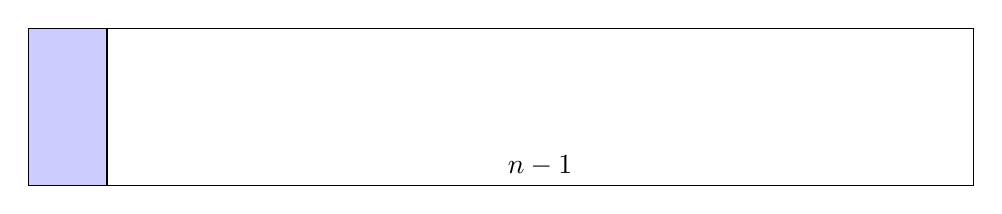
\begin{tikzpicture}

\draw (6.0, 1.0)
  node[draw, , , color=black,
       rounded corners=0cm, inner sep=0cm] {

\begin{minipage}[t][2cm]{12cm}
\mbox{}

\end{minipage}

};
\draw (0.5, 1.0)
  node[fill=blue!20!white,rounded corners=0cm,inner sep=0cm] {

\begin{minipage}[t][2cm]{1cm}
\mbox{}

\end{minipage}

};
\draw (0.5, 1.0)
  node[draw, , , color=black,
       rounded corners=0cm, inner sep=0cm] {

\begin{minipage}[t][2cm]{1cm}
\mbox{}

\end{minipage}

};
\draw (6.5, 0.25)
  node[draw=none, line width=0cm, , color=black,
       rounded corners=0cm, inner sep=0cm] {

\begin{minipage}[t][0.1cm]{0.1cm}
\mbox{}

\end{minipage}

};\draw (6.5, 0.25) node[color=black] {$n - 1$};
\end{tikzpicture}

\end{center}



Draw an ${\large \times}$ when a machine crashes.
Then you let the machine at $q_0$ and $q_4$
spawn off new machines along $epsilon$--transitions, 
drawing the $\epsilon$-arrows vertically again:

\begin{center}
\begin{tikzpicture}

\fill[blue!10] (0.0, 0.0) circle (0.3);
\node [line width=0.03cm,black,minimum size=0.57cm,draw,circle] at (0.0,0.0)(a){};\draw (0.0, 0.0) node[color=black] {$a$};
\fill[blue!10] (-2.0, -1.0) circle (0.3);
\node [line width=0.03cm,black,minimum size=0.57cm,draw,circle] at (-2.0,-1.0)(b){};\draw (-2.0, -1.0) node[color=black] {$b$};
\fill[blue!10] (2.0, -1.0) circle (0.3);
\node [line width=0.03cm,black,minimum size=0.57cm,draw,circle] at (2.0,-1.0)(d){};\draw (2.0, -1.0) node[color=black] {$d$};
\fill[blue!10] (-3.0, -2.0) circle (0.3);
\node [line width=0.03cm,black,minimum size=0.57cm,draw,circle] at (-3.0,-2.0)(e){};\draw (-3.0, -2.0) node[color=black] {$e$};
\fill[blue!10] (-1.0, -2.0) circle (0.3);
\node [line width=0.03cm,black,minimum size=0.57cm,draw,circle] at (-1.0,-2.0)(f){};\draw (-1.0, -2.0) node[color=black] {$f$};
\fill[blue!10] (1.0, -2.0) circle (0.3);
\node [line width=0.03cm,black,minimum size=0.57cm,draw,circle] at (1.0,-2.0)(m){};\draw (1.0, -2.0) node[color=black] {$m$};
\fill[blue!10] (3.0, -2.0) circle (0.3);
\node [line width=0.03cm,black,minimum size=0.57cm,draw,circle] at (3.0,-2.0)(o){};\draw (3.0, -2.0) node[color=black] {$o$};
\fill[blue!10] (-3.5, -3.0) circle (0.3);
\node [line width=0.03cm,black,minimum size=0.57cm,draw,circle] at (-3.5,-3.0)(k){};\draw (-3.5, -3.0) node[color=black] {$k$};
\fill[blue!10] (-2.5, -3.0) circle (0.3);
\node [line width=0.03cm,black,minimum size=0.57cm,draw,circle] at (-2.5,-3.0)(l){};\draw (-2.5, -3.0) node[color=black] {$l$};
\fill[blue!10] (3.5, -3.0) circle (0.3);
\node [line width=0.03cm,black,minimum size=0.57cm,draw,circle] at (3.5,-3.0)(j){};\draw (3.5, -3.0) node[color=black] {$j$};\draw[line width=0.03cm,black,->,>=triangle 60] (a) to  (b);
\draw[line width=0.03cm,black,->,>=triangle 60] (a) to  (d);
\draw[line width=0.03cm,black,->,>=triangle 60] (b) to  (e);
\draw[line width=0.03cm,black,->,>=triangle 60] (b) to  (f);
\draw[line width=0.03cm,black,->,>=triangle 60] (d) to  (m);
\draw[line width=0.03cm,black,->,>=triangle 60] (d) to  (o);
\draw[line width=0.03cm,black,->,>=triangle 60] (e) to  (k);
\draw[line width=0.03cm,black,->,>=triangle 60] (e) to  (l);
\draw[line width=0.03cm,black,->,>=triangle 60] (o) to  (j);
\end{tikzpicture}

\end{center}



Repeat. You will find this more organized and harder to miss things.

\begin{defn}
If the NFA is denoted $N$, then $L(N)$ is the language accepted by
$N$, in other words $L(N)$ is the set of \textbf{all} strings over
$\Sigma$ accepted by $N$.
\end{defn}

%-*-latex-*-

\begin{ex} 
  \label{ex:prob-00}
  \tinysidebar{\debug{exercises/{disc-prob-28/question.tex}}}

  \solutionlink{sol:prob-00}
  \qed
\end{ex} 
\begin{python0}
from solutions import *
add(label="ex:prob-00",
    srcfilename='exercises/discrete-probability/prob-00/answer.tex') 
\end{python0}


%-*-latex-*-

\begin{ex} 
  \label{ex:prob-00}
  \tinysidebar{\debug{exercises/{disc-prob-28/question.tex}}}

  \solutionlink{sol:prob-00}
  \qed
\end{ex} 
\begin{python0}
from solutions import *
add(label="ex:prob-00",
    srcfilename='exercises/discrete-probability/prob-00/answer.tex') 
\end{python0}


%-*-latex-*-

\begin{ex} 
  \label{ex:prob-00}
  \tinysidebar{\debug{exercises/{disc-prob-28/question.tex}}}

  \solutionlink{sol:prob-00}
  \qed
\end{ex} 
\begin{python0}
from solutions import *
add(label="ex:prob-00",
    srcfilename='exercises/discrete-probability/prob-00/answer.tex') 
\end{python0}


%-*-latex-*-

\begin{ex} 
  \label{ex:prob-00}
  \tinysidebar{\debug{exercises/{disc-prob-28/question.tex}}}

  \solutionlink{sol:prob-00}
  \qed
\end{ex} 
\begin{python0}
from solutions import *
add(label="ex:prob-00",
    srcfilename='exercises/discrete-probability/prob-00/answer.tex') 
\end{python0}


%-*-latex-*-

\begin{ex} 
  \label{ex:prob-00}
  \tinysidebar{\debug{exercises/{disc-prob-28/question.tex}}}

  \solutionlink{sol:prob-00}
  \qed
\end{ex} 
\begin{python0}
from solutions import *
add(label="ex:prob-00",
    srcfilename='exercises/discrete-probability/prob-00/answer.tex') 
\end{python0}


%-*-latex-*-

\begin{ex} 
  \label{ex:prob-00}
  \tinysidebar{\debug{exercises/{disc-prob-28/question.tex}}}

  \solutionlink{sol:prob-00}
  \qed
\end{ex} 
\begin{python0}
from solutions import *
add(label="ex:prob-00",
    srcfilename='exercises/discrete-probability/prob-00/answer.tex') 
\end{python0}


%-*-latex-*-

\begin{ex} 
  \label{ex:prob-00}
  \tinysidebar{\debug{exercises/{disc-prob-28/question.tex}}}

  \solutionlink{sol:prob-00}
  \qed
\end{ex} 
\begin{python0}
from solutions import *
add(label="ex:prob-00",
    srcfilename='exercises/discrete-probability/prob-00/answer.tex') 
\end{python0}


%-*-latex-*-

\begin{ex} 
  \label{ex:prob-00}
  \tinysidebar{\debug{exercises/{disc-prob-28/question.tex}}}

  \solutionlink{sol:prob-00}
  \qed
\end{ex} 
\begin{python0}
from solutions import *
add(label="ex:prob-00",
    srcfilename='exercises/discrete-probability/prob-00/answer.tex') 
\end{python0}


%-*-latex-*-

\begin{ex} 
  \label{ex:prob-00}
  \tinysidebar{\debug{exercises/{disc-prob-28/question.tex}}}

  \solutionlink{sol:prob-00}
  \qed
\end{ex} 
\begin{python0}
from solutions import *
add(label="ex:prob-00",
    srcfilename='exercises/discrete-probability/prob-00/answer.tex') 
\end{python0}


%-*-latex-*-

\begin{ex} 
  \label{ex:prob-00}
  \tinysidebar{\debug{exercises/{disc-prob-28/question.tex}}}

  \solutionlink{sol:prob-00}
  \qed
\end{ex} 
\begin{python0}
from solutions import *
add(label="ex:prob-00",
    srcfilename='exercises/discrete-probability/prob-00/answer.tex') 
\end{python0}


%-*-latex-*-

\begin{ex} 
  \label{ex:prob-00}
  \tinysidebar{\debug{exercises/{disc-prob-28/question.tex}}}

  \solutionlink{sol:prob-00}
  \qed
\end{ex} 
\begin{python0}
from solutions import *
add(label="ex:prob-00",
    srcfilename='exercises/discrete-probability/prob-00/answer.tex') 
\end{python0}


%-*-latex-*-

\begin{ex} 
  \label{ex:prob-00}
  \tinysidebar{\debug{exercises/{disc-prob-28/question.tex}}}

  \solutionlink{sol:prob-00}
  \qed
\end{ex} 
\begin{python0}
from solutions import *
add(label="ex:prob-00",
    srcfilename='exercises/discrete-probability/prob-00/answer.tex') 
\end{python0}


%-*-latex-*-

\begin{ex} 
  \label{ex:prob-00}
  \tinysidebar{\debug{exercises/{disc-prob-28/question.tex}}}

  \solutionlink{sol:prob-00}
  \qed
\end{ex} 
\begin{python0}
from solutions import *
add(label="ex:prob-00",
    srcfilename='exercises/discrete-probability/prob-00/answer.tex') 
\end{python0}

